%!TEX root = ../Thesis.tex
%Chapter 3

\chapter{Quantum-Optical implementation of non-Hermitian potentials for asymmetric scattering}
\label{Chapter3}
\lhead{Chapter 3. \emph{Quantum-Optical implementation of non-Hermitian potentials for asymmetric scattering}}

In chapter \ref{Chapter1}, non-local potentials for asymmetric scattering had been constructed as mathematical models but without a physical implementation. In this chapter a feasible quantum-optical implementation
of non-Hermitian, non-local, non-PT potentials is put forward to implement different scattering asymmetries, including transmission
asymmetries. Using Feshbach's projection technique it is found that the effective potentials for a ground-state atom crossing a laser beam in a region of space are generically non-local and non-Hermitian. Shaping the spatial-dependence of the, generally complex, Rabi frequency, and selecting a specific laser detuning allows to produce different potential symmetries and asymmetric scattering effects, including asymmetric transmission.

The rest of this chapter is organized as follows. In Sec. \ref{sec:chapter3_enl}, I shall explain how to generate different NH symmetries in a quantum optical setting of an atom impinging on a laser illuminated region. In Sec. \ref{sec:chapter3_exa}, I provide specific example devices (constructed using numerical optimisation) with different asymmetric scattering responses. Realistic experimental parameters are also examined. In Sec. \ref{sec:chapter3_class}, the asymmetric behavior is explained with a classical approximation of the motion and the non-commutativity of rotations on the Bloch sphere, which gives good estimates for the potential parameters. Finally, in Sec. \ref{sec:chapter3_Discussion} I summarize the main findings in the chapter.

%---------------------------------------------------------------------------------------------
\begin{table}[t]
  \caption{Conditions leading to  specific symmetries in the potential \eqref{eq:chapter3_effpot}. A given symmetry also implies others, see the last column.\label{tab:chapter3_SymmetriesConditions}}
  \hspace*{-0.1cm}
  \centering
  \begin{tabular}{lcc}
  \hline\hline
  Symmetry& Conditions & Implies
  \\
  \hline
  (I)\;$1H=H1$ &   none & -
  \\
  (II)\;$1H=H^\dagger 1$ &  $q=-q^{*}$ (i.e. $\operatorname{Re}q=0$) & I
  \\
  (III)\;$ \Pi H=H\Pi$ &  $\Omega(x)=e^{i\phi}\Omega(-x)$ & I
  \\
  (IV) $\Pi H=H^\dagger \Pi$ &  $q=-q^{*}$ \& $\Omega(x)=e^{i\phi}\Omega(-x)$ & III,\! II,\! I
  \\
  (V) $\Theta H=H\Theta$ &  $q=-q^{*}$ \& $\Omega(x)=e^{i\phi}\Omega(x)^*$ & {\small VI,\! II,\! I}
  \\
  (VI) $\Theta H=H^\dagger\Theta$ &  $\Omega(x)=e^{i\phi}\Omega(x)^*$ & I
  \\
  (VII) $\Theta\Pi H=H\Theta \Pi$ &  $q=-q^{*}$ \& $\Omega(x)=e^{i\phi}\Omega(-x)^*$ & VIII,\! II,\! I
  \\
  (VIII)\,$\Theta\Pi H=H^\dagger \Theta \Pi$ &  $\Omega(x)=e^{i\phi}\Omega(-x)^*$  & I
  \\
  \hline\hline
  \end{tabular}
\end{table}
%---------------------------------------------------------------------------------------------

%
\section{Effective non-local potential for the ground state of a two-level atom\label{sec:chapter3_enl}}
%
The key task is to physically realize some of the potential and asymmetric device types described in chapter \ref{Chapter1}, which are again summarized in table \ref{tab:chapter3_table2PhysicalImplementation}. I start with a two-level atom with ground level $\ket{1}$ and excited state $\ket{2}$ impinging onto a laser illuminated region. For a full account of the model and further references see
\cite{Ruschhaupt2009}. The motion is assumed one dimensional, either because the atom is confined in a waveguide or because the direction $x$ is uncoupled to
the others.
I only account explicitly for atoms before the first spontaneous emission in the wavefunction
\cite{Hegerfeldt1996,Damborenea2002,Navarro2003}.
If the excited atom emits a spontaneous photon it disappears from the coherent wavefunction ensemble.
I assume that no resetting into the ground state occurs. The physical mechanism
may be an irreversible decay into a third level  \cite{Oberthaler1996}, or atom ejection from the waveguide or the privileged 1D direction due to  random recoil  \cite{Streed2006}.
The state ${\bf\Phi}_k=\left(\begin{smallmatrix}\phi_k^{(1)},\phi_k^{(2)}\end{smallmatrix}\right)^{\sf T}$
for the atom before the first spontaneous emission impinging with wavenumber $k$
in a laser adapted  interaction picture,
obeys, after applying the rotating wave approximation, an effective stationary Schr\"{o}dinger equation
with a time-independent Hamiltonian \cite{Ruschhaupt2004a,Ruschhaupt2009}
%
${\cal H}{\bf\Phi}_k(x)=E{\bf\Phi}_k(x)$,
%
where
%
\begin{eqnarray}
  {\cal H}&=& H_0{\bf 1}+ {\cal V}=\frac{1}{2m}\left(
  {{p}^2\atop 0}{0\atop {p}^2}\right)+ {\cal V}(x),
  \\
  {\cal V}(x) &=&
  \frac{\hbar}{2}\left(
  {0\atop \Omega(x)^*}\;\;\;\;
  {\Omega(x)\atop -(2\Delta+i\gamma)}
  \right).
\end{eqnarray}
%
I assume perpendicular incidence of the atom on the laser sheet for simplicity, oblique incidence is treated e.g. in  \cite{Ruschhaupt2007,Ruschhaupt2009}.
Here $E=\hbar^2 k^2/2m$ is the energy, and
$\Omega(x)$ is the position-dependent, on-resonance Rabi frequency, where real and imaginary parts may be controlled independently
using two  laser field quadratures  \cite{Zhang2013};
$\gamma$ is the inverse of the life time of the excited state;
$\Delta=\omega_{L}-\omega_{12}$
is the detuning (laser angular frequency minus the atomic transition
angular frequency $\omega_{12}$);
${p}=-i\hbar\partial/\partial x$ is the momentum operator;
and ${\bf 1}=|1\ra\la 1|+|2\ra\la 2|$ is the unit operator
for the internal-state space.
Complementary projectors
%
$P=|1\ra\la 1|$ and $Q=|2\ra\la 2|$
%
are defined to select ground and excited state components.
Using the Feshbach partitioning
technique \cite{Feshbach1958,Feshbach1962,Levine1969},
I find for the ground
state amplitude $\phi_k^{(1)}$ the equation
%
\begin{equation}\label{effecti}
  E\phi_k^{(1)}(x) = H_0\phi_k^{(1)}(x)+\!
  \int\! dy\, \la x,1|{\cal W}(E)|y,1\ra \phi_k^{(1)}(y),
\end{equation}
%
where
%
$
{\cal W}(E)=P{\cal V}P+P{\cal V}Q(E+i0-Q{\cal H}Q)^{-1}Q{\cal V}P,
$
%
is generically non local and energy dependent. Specifically, I have now achieved
a physical realization of an effective (in general) non-local, non-Hermitian potential whose kernel has the form
%
\begin{eqnarray}
  \hspace*{-.3cm}V (x,y) = \la x,1|{\cal W}(E)|y,1\ra = \frac{m}{4} \frac{e^{i|x-y|q}}{i q}
  \Omega(x)\Omega(y)^*,
  \label{eq:chapter3_effpot}
\end{eqnarray}
%
%
where
$
q=\frac{\sqrt{2mE}}{\hbar}(1+\mu)^{1/2},\;\;
{\rm Im}\,q\ge 0,
\label{qeq}
$ and
$
\mu=\frac{2\Delta+i\gamma}{2E/\hbar}.
$
%
Eq. \eqref{eq:chapter3_effpot} is worked out  in momentum representation to do the integral
using the residue theorem.
This is a generalized, non-local version of the effective potentials known for the ground state
\cite{Chudesnikov1991,Oberthaler1996}, which are found from Eq. \eqref{eq:chapter3_effpot}  in the large $\mu$ limit \cite{Ruschhaupt2004a}.
The reflection and transmission amplitudes $R^{r,l}$ and  $T^{r,l}$ may be calculated directly
using the potential \eqref{eq:chapter3_effpot} or as corresponding amplitudes for
transitions from ground state to ground state in the full two-level theory (see Appendix \ref{Appendix:NumericalCalculationOfTandR}).

%%%%%%%%%
\begin{table}
  \caption{Device types for  transmission and/or reflection asymmetry in the first row (see Sec. \ref{sec:chapter1_AsymmetricDevices} for nomenclature).
  The second row gives the corresponding symmetries  that allow
  each device.
  \label{devices}}
  \vspace*{.0cm}
  \label{tab:chapter3_table2PhysicalImplementation}
  \centering
  \begin{tabular}{cccccc}
    \hline\hline
    $\cal{TR/A}$ & $\cal{T/R}$ & $\cal{T/A}$ & $\cal{TR/R}$ & $\cal{R/A}$ & $\cal{TR/T}$ \\
    \hline
    I            & I           & I,VIII      & I,VIII       & I,VI        & I, IV, VI, VII
    \\
    \hline\hline
  \end{tabular}
\end{table}
%

\subsection{Possible symmetries of the non-local potential}
%
The necessary conditions for the different symmetries of a non-Hermitian and non-local Hamiltonian were worked out in Sec. \ref{sec:chapter1_AsymmetricDevices}. In the second column of table \ref{tab:chapter3_SymmetriesConditions}, those conditions have been particularized for the effective potential of the 2-level atom \eqref{eq:chapter3_effpot}. For example, symmetry III (parity) requires that $V(x,y)=V(-x,-y)$ (see table \ref{tab:chapter1_SymmetriesTable}). Inserting the functional form of the potential from Eq. \eqref{eq:chapter3_effpot} into this condition, it results in the requirement $\Omega(x) \Omega(y)^* = \Omega(-x) \Omega(-y)^*$. This is fulfilled if $\Omega(x)=\Omega(-x)e^{i \phi}$ with some arbitrary phase freedom $\phi$.

Since $\Omega(x)$ does not depend on $q$, symmetries IV, V and VII imply that symmetry II is obeyed as well (Hermiticity).
Moreover symmetry III (parity) should be discarded for our purpose since it does not allow for asymmetric transmission or reflection
\cite{Ruschhaupt2017}.
This leaves us with three interesting symmetries to explore:
VI, which allows for  asymmetric reflection; VIII which allows for asymmetric transmission, and  I,
which in principle allows for arbitrary asymmetric responses, except for physical limitations imposed by
the two-level model see Appendix \ref{Appendix:NumericalCalculationOfTandR}.

As seen from  table \ref{tab:chapter3_SymmetriesConditions}, $\operatorname{Re}(q)=0$ makes the potential Hermitian, so it must be avoided.
If $\gamma=0$,   $\mu \in \mathbb{R}$. Hence $\mu+1<0$ gives $\operatorname{Re}(q)=0$ and $\mu+1>0$ gives
$\operatorname{Im}(q)=0$. $\mu+1>0$ amounts to a condition on the detuning compared to the incident energy, namely $\Delta>-E/\hbar$.
In the following examples I implement potentials with symmetries VIII, VI, and I, with detunings and energies satisfying the condition $\mu+1>0$.


\section{Design of asymmetric devices\label{sec:chapter3_exa}}

I will now apply this method to physically realize non-local potentials of the form \eqref{eq:chapter3_effpot}. I shall work out explicitly a ${\cal T/A}$ device with symmetry  VIII, a ${\cal R/A}$ device with symmetry  VI, and a ``partial''-${\cal TR/A}$ device,  having 1/2 transmission and reflection coefficients from the left, with symmetry I. The  ${\cal T/A}$ and the ``partial''-${\cal TR/A}$ device have transmission asymmetry so they cannot be built with local or $PT$-symmetric  potentials.
%, whereas   to design asymmetric devices which can be shown not to be implementable with a one-dimensional, one-channel, local potential.
Let us  motivate the effort with some possible applications, relations  and analogies of these devices.
${\cal T/A}$ and ${\cal R/A}$ are, respectively, transmission and reflection filters. They are analogous to
half-wave electrical rectifiers that either let the signal from one side ``pass'' (transmitted) or change its sign (reflected)
while suppressing the other half signal.  They may play the role of half-rectifiers in atomtronic circuits.
A ${\cal T/A}$ device allows us, for example, to empty a region of selected particles, letting them go away while not letting particles in.
The ``atom diode'' devices worked out e.g. in \cite{Ruschhaupt2004,Ruschhaupt2006a,Ruschhaupt2006,Ruschhaupt2007}
where of type ${\cal R/A}$. As the mechanism behind them was adiabatic, a broad range of momenta with the desired asymmetry
could be achieved. In comparison the current approach is not necessarily adiabatic so it can be adapted to faster processes.

As for the ``partial''-${\cal RT/A}$ device,  it reflects and transmits from one side while absorbing from the
other side. In an optical analogy an observer from the left perceives it as a darkish mirror.
An observer from the right ``sees'' the other side because of the allowed transmission
but cannot be seen from the left since  nothing is transmitted from right to left. Our device is necessarily ``partial'' one as
there cannot be  net probability gain because of the underlying two-level system, and a ``full'' version with both reflection and transmission coefficients equal to one
would need net gain.

The three devices are worked out for $\gamma=0$, a valid approximation for  hyperfine transitions. %, although this is by no means a necessary assumption.
I assume for the Rabi frequencies the forms
%
\begin{eqnarray}
  \Omega_{\rm VIII} (x) &=& a [g(x+x_0) + i  g(x-x_0)],
  \nonumber\\
  \Omega_{\rm VI} (x) &=&  b g(x+x_0) + c g(x-x_0),
  \nonumber\\
  \Omega_{\rm I} (x) &=&  - i b g(x+x_0) + c g(x-x_0),
  \label{3omegas}
\end{eqnarray}
%
in terms of smooth, realizable Gaussians $g(x) =  \exp[-{x^2}/{w^2}]$.
I fix $2 d$ as an effective finite width
of the potential area beyond which the potential is negligible and assumed to vanish. I will express in the following the different length parameters as a multiple of $d$ to keep results general.
In addition, I will use as a scaling factor for the velocity $v_{d} = {\hbar}/({m d})$, and for time $\tau={m d^2}/{\hbar}$.

In the following calculations I fix the width of the Gaussians to be $w= {\sqrt{2}}d/{10}$.
I always first set a target velocity $v_0$ to achieve the desired asymmetric scattering response.
The real parameters $a$, $b$, $c$, $x_0$ in Eq. \eqref{3omegas}, and  $\Delta$
are then numerically optimized with the GRAPE (Gradient Ascent Pulse Engineering) algorithm \cite{Khaneja2005,Wu2015}.

The Rabi frequencies will fulfill the indicated symmetries VIII, VI, and I. $\Omega_{\rm VI}(x)$ should not be even (i.e. $b \neq c$) to avoid symmetry II. In addition, $\Omega_{\rm I}(x)$ should not fulfill any other symmetry than ${\rm I}$.
The corresponding Rabi frequencies $\Omega(x)$ are  depicted in Figs. \ref{fig_t_a}, top row.
The scattering coefficients are shown in the bottom row. Fig. \ref{fig_t_a} demonstrates that the three potentials satisfy the asymmetric response conditions imposed
at the selected velocity and also in a region nearby.

The ``partial''-${\cal TR/A}$  device fullfills $\absq{T^l} = \absq{R^l} = 1/2$ and full absorption from the right.
The potential I use for that device has symmetry I only, i.e., ``no symmetry'' other than the trivial commutation with the identity. No other potential symmetry would allow this type of device.

The effective non-local potential $V(x,y)$, see Eq. \eqref{eq:chapter3_effpot}, corresponding to the $v/v_d$ ratios used for the three devices is shown in Fig. \ref{fig_poten1}. Note that the non-local potential has dimensions  energy/length, so  we
divide the absolute value by a factor $V_0=\hbar^2/(m d^3)$ to plot a dimensionless quantity.


% -------------------------------------------------------------
\begin{figure}
  \begin{center}
  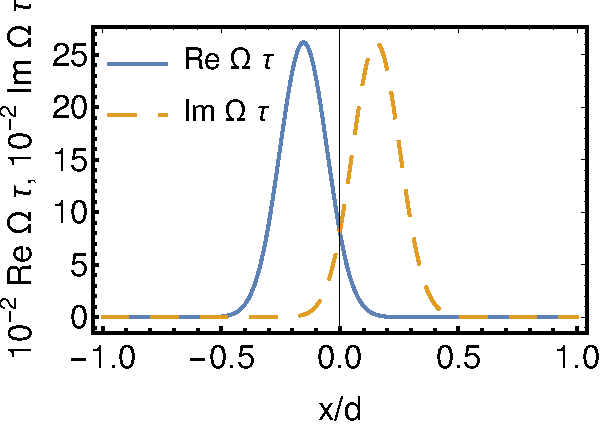
\includegraphics[width=0.28\linewidth]{Figures/asym_fig_t_a_400_pot.pdf}
  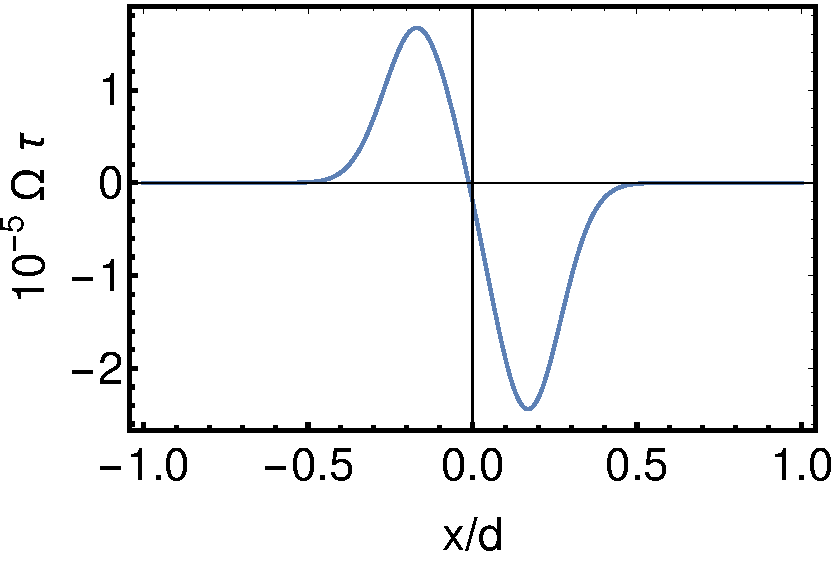
\includegraphics[width=0.28\linewidth]{Figures/asym_fig_r_a_400_pot.pdf}
  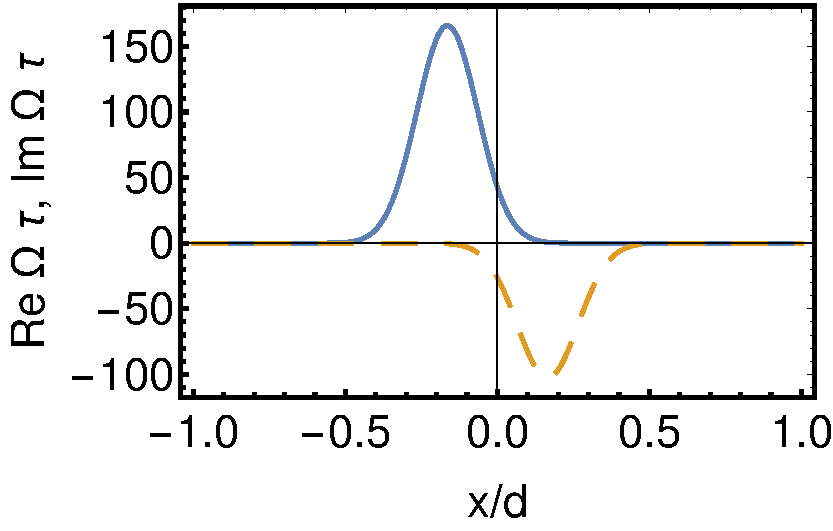
\includegraphics[width=0.28\linewidth]{Figures/asym_fig_1_2_tr_a_8_pot.pdf}\\
  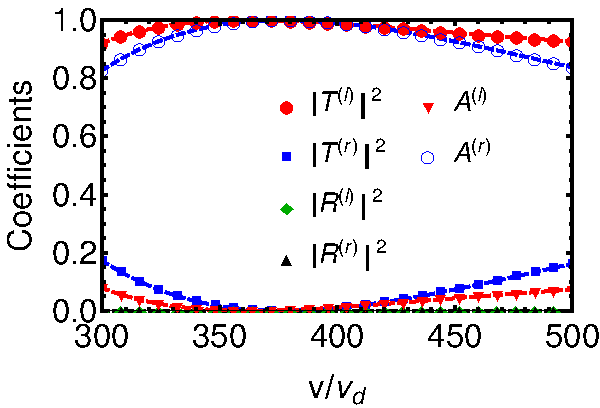
\includegraphics[width=0.29\linewidth]{Figures/asym_fig_t_a_400.pdf}
  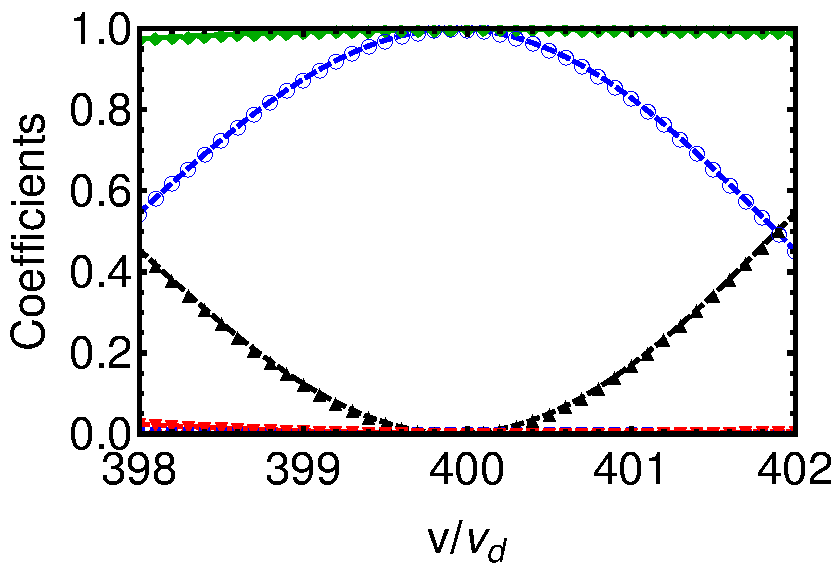
\includegraphics[width=0.29\linewidth]{Figures/asym_fig_r_a_400.pdf}
  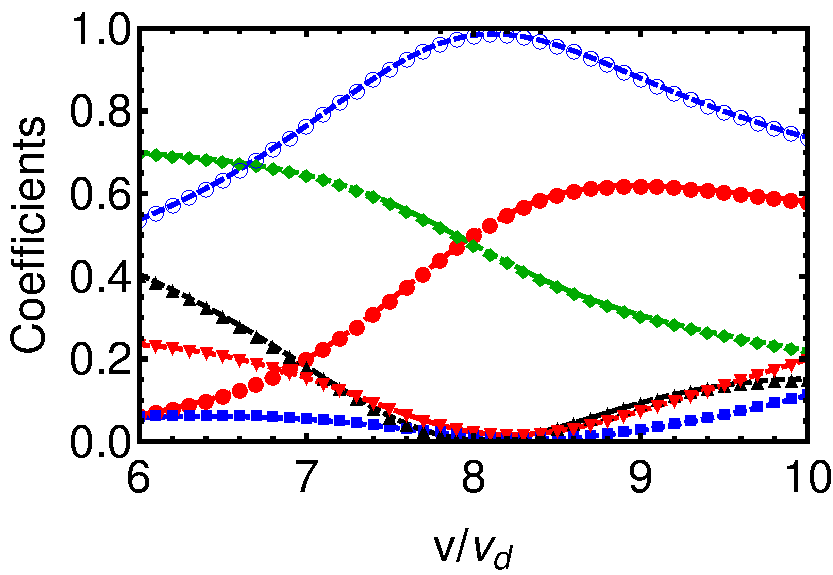
\includegraphics[width=0.29\linewidth]{Figures/asym_fig_1_2_tr_a_8.pdf}
  \end{center}
  \caption{Left column: ${\cal T/A}$ device with symmetry VIII.
  Top: $\Omega_{\rm VIII}(x)$;
  Bottom:  transmission and reflection coefficients. $v_0/v_d=400$, $a\tau = 2618.19$,
  $x_0/d = 0.1532$, $\tau\Delta = 1413.01$.
  %
  Middle column: ${\cal R/A}$ device with symmetry VI.
  Top: $\Omega_{\rm VI} (x)$ (it is real); Bottom:  transmission and reflection coefficients. $v_0/v_d=400$,
  $b \tau =  -244516.1$,
  $c\tau = 167853.9$,
  $x_0/d = 0.1679$,
  $\tau\Delta= 193.508$.
  %
  Right column: ``Partial''-${\cal TR/A}$ device with symmetry I.
  Top:  $\Omega_{\rm I}(x)$, real (blue, solid line) and imaginary parts (orange, dashed line);
  Bottom: transmission and reflection coefficients. $v_0/v_d=8$, $b\tau =  102.6520$,
  $c \tau =  165.8355$,
  $x_0/d = 0.1648$,
  $\tau\Delta= 90.5337$. In all cases $\tau={m d^2}/{\hbar}$ and $v_{d} = {\hbar}/({m d})$.
  \label{fig_t_a}}
\end{figure}
% -------------------------------------------------------------

%--------------------------------------------------------------------------
\begin{figure}
  \begin{center}
  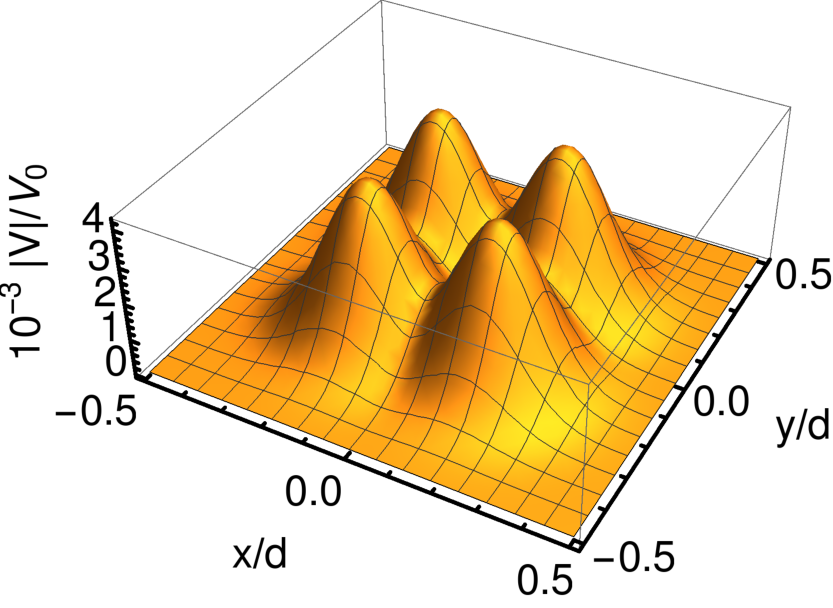
\includegraphics[width=0.28\linewidth]{Figures/asym_fig_t_a_400_eff_pot_abs.pdf}
  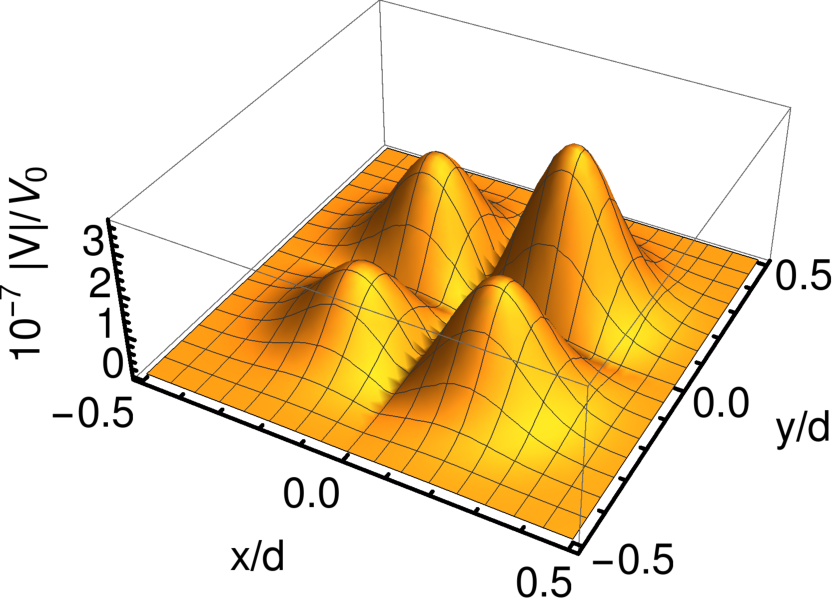
\includegraphics[width=0.28\linewidth]{Figures/asym_fig_r_a_400_eff_pot_abs.pdf}
  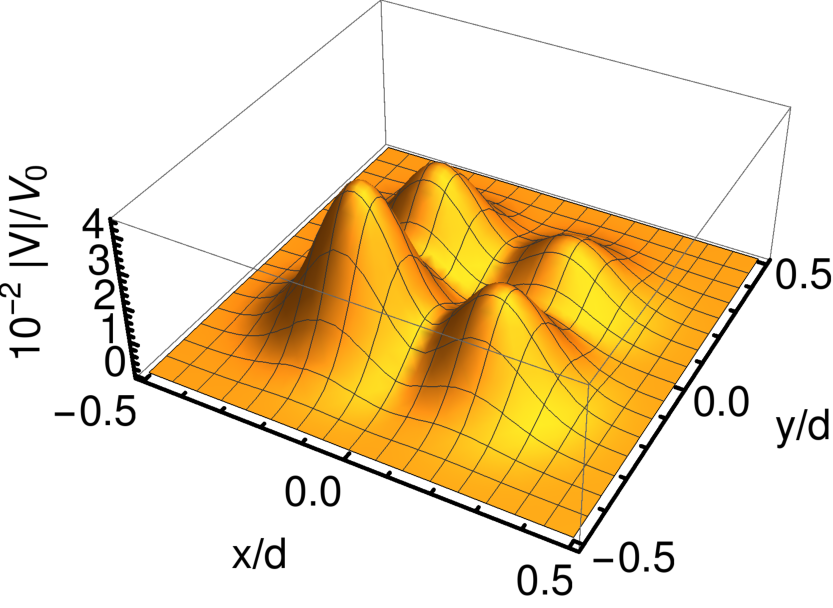
\includegraphics[width=0.28\linewidth]{Figures/asym_fig_1_2_tr_a_8_eff_pot_abs.pdf}\\
  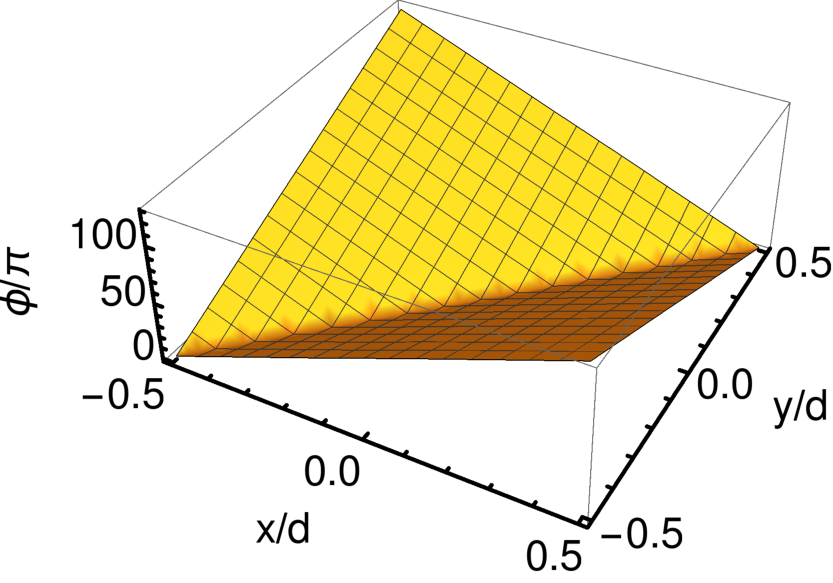
\includegraphics[width=0.29\linewidth]{Figures/asym_fig_t_a_400_eff_pot_arg.pdf}
  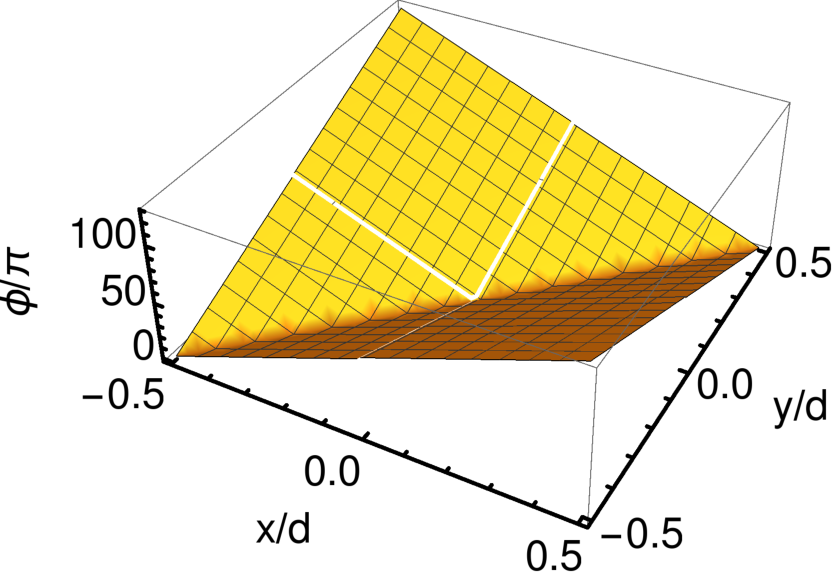
\includegraphics[width=0.29\linewidth]{Figures/asym_fig_r_a_400_eff_pot_arg.pdf}
  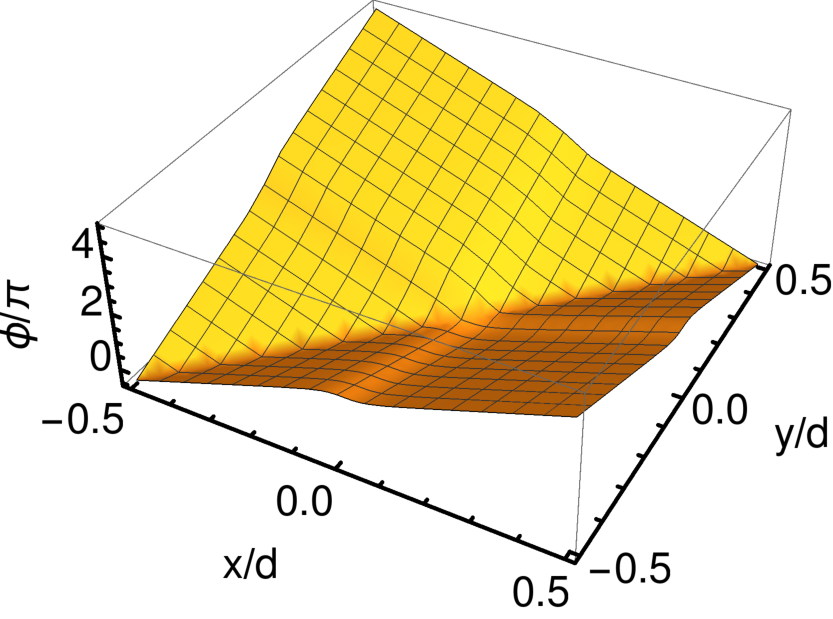
\includegraphics[width=0.29\linewidth]{Figures/asym_fig_1_2_tr_a_8_eff_pot_arg.pdf}
  \end{center}
  \caption{Nonlocal potentials  $V(x,y)$: absolute value (top), argument (bottom).
  Left column: Potential for ${\cal T/A}$ device with symmetry VIII.
  Middle column: Potential for ${\cal R/A}$ device with symmetry VI.
  Right column: ``Partial''-${\cal TR/A}$ device with symmetry I.
  $V_0=\hbar^2/(md^3)$.}
  \label{fig_poten1}
\end{figure}
%--------------------------------------------------------------------------

In the parameter optimization I see that increasing the velocities further does not pose a problem for the ${\cal T/A}$
device, it is more challenging for a ${\cal R/A}$ device, and it is quite difficult for the partial-${\cal RT/A}$ device.  The device ${\cal T/A}$ is feasible for an experimental implementation  as the ratio $v_0/v_d$ can be easily increased to desired values, for  reasonable values of the
Rabi frequency and laser waist \cite{Zeyen2016}.

Moreover the velocity width with the desired behavior is much broader for ${\cal T/A}$. Therefore a ${\cal T/A}$
device is the best candidate for
an experimental implementation.
As a check of feasibility, let us assume a Beryllium ion. Its hyperfine structure provides a good  two-level system
for which I can neglect decay (i.e. $\gamma\approx 0$ is indeed realistic). I have $m=1.49\times 10^{-26}$ kg
and set a length $d=10\, \mu$m compatible with the small laser waists (in this case 1.4 $\mu$m) achieved for individual ion
addressing \cite{Zeyen2016}. The scaling factors take the values
%
\begin{eqnarray}
  v_d&=&0.67\, {\rm mm/s},
  \nonumber\\
  \tau&=&1.49\times 10^{-2}\, {\rm s},
  \nonumber
\end{eqnarray}
%
which gives  $v\approx$ 27 cm/s for $v/v_d=400$, (again, I see no major obstacle to get devices for higher velocities,
in particular the classical approximations in Sec. \ref{sec:chapter3_class} can be used to  estimate the values of the parameters)
and Rabi frequencies, see Fig. \ref{fig_t_a},  in the hundreds of kHz range. The relative ion-laser beam velocity could be as well
implemented  by moving the beam in the laboratory frame.

%
%
\section{Classical approximation for ${\cal T/A}$ device \label{sec:chapter3_class}}
%
%
In a ${\cal T/A}$ device such as the one presented an incident plane wave from the left ends up as a pure transmitted wave with no reflection or absorption.
However, a wave incident from the right is fully absorbed. How can that be? Should not the velocity-reversed motion
of the transmitted wave lead to the reversed incident wave?
%Obviously that is not the case, and a formal answer to that question  is that $V$ is not time-reversal invariant.
For a more intuitive understanding I may seek help in the underlying two-level model.
In the larger space the potential is again local and Hermitian. A simple semiclassical
approximation is to assume that the particle moves with  constant speeds $\pm v$ for left ($v>0$) or right ($-v<0$) incidence,  so that at a given time it is subjected to  the $2\times2$ time-dependent potentials
${\cal V}(\pm vt)$. The incidence from the left and right give different time dependences for the potential. The scattering problem then reduces to solving the time-dependent Schr\"odinger equation for the amplitudes of a two-level atom with time-dependent potential, i.e. to solving the following time-dependent Schr\"odinger equation ($\gamma = 0$)
%
\begin{eqnarray}
  i \hbar \frac{\partial}{\partial t} \chi_\pm(t)
  = {\cal V} (\pm v t) \chi_\pm(t),
\end{eqnarray}
%
with the appropriate boundary conditions $\chi_+ (-\infty) = \chi_- (-\infty) =\left(\begin{smallmatrix} 1\\ 0\end{smallmatrix}\right)$. The  solutions for $v/v_d = 400$
%9.1
are shown in Fig. \ref{fig_t_a_approx}.
In Fig. \ref{fig_t_a_approx}(a), $\chi_+ (t)$ (left incidence) is depicted:  the particle ends  with high probability in the ground state at final time. In Fig. \ref{fig_t_a_approx}(b), $\chi_- (t)$ (right incidence) demonstrates  the ground state population is transferred to the excited state. Projected onto the ground-state level alone,
this corresponds to full absorption of the ground state population at final time.

For an  even rougher but also illustrative picture,  again in a semiclassical time-dependent framework, I  may substitute the smooth Gaussians for Re$(\Omega)$ and Im$(\Omega)$ in Fig. \ref{fig_t_a} by two simple, contiguous square functions of height
$\Omega>0$ and width $\tilde{w} > 0$. Then, the $2\times2$ potential at a given time is, in terms of Pauli matrices,
%
\begin{eqnarray}
  {\cal V} (x) = \frac{\hbar}{2}\Delta (\sigma_Z-{\mathbf 1})+ \frac{\hbar}{2} \left\{\begin{array}{cc}
  \Omega\sigma_X & -\tilde w < x < 0\\
  -\Omega\sigma_Y & 0 < x < \tilde w\\
  0 & \mbox{otherwise}
  \end{array}\right.
\end{eqnarray}
%
where $x = \pm v t$ and let ${\sf T}=2 \tilde w/v$.

% ------------------------------------------------------------------------------
\begin{figure}
  \begin{center}
  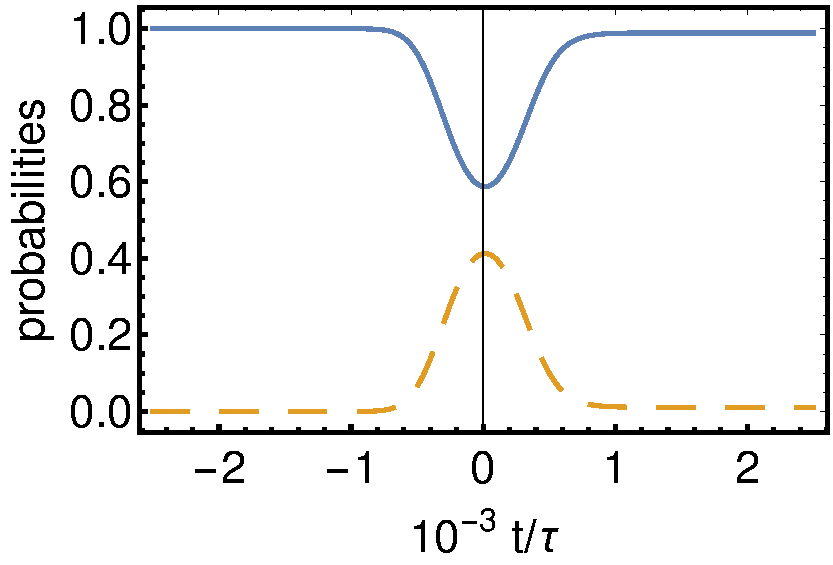
\includegraphics[width=0.48\linewidth]{Figures/asym_fig_t_a_approx_left.pdf}
  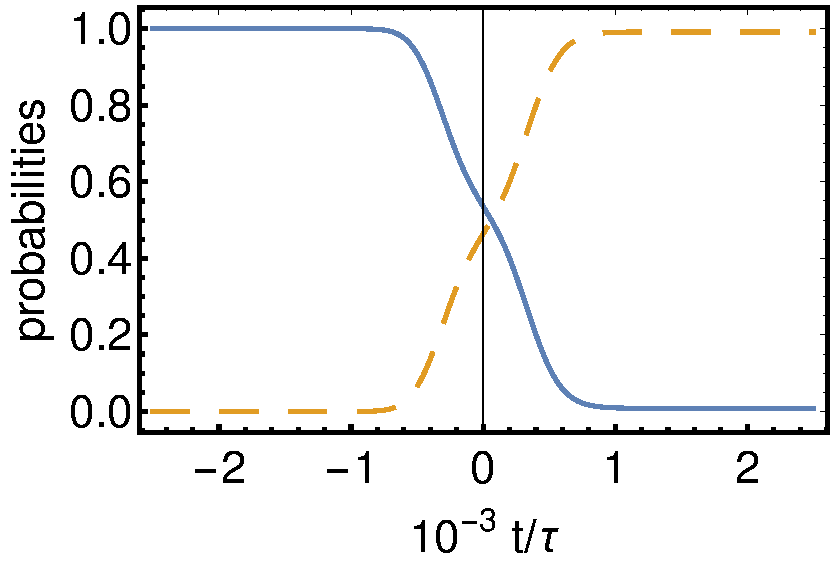
\includegraphics[width=0.48\linewidth]{Figures/asym_fig_t_a_approx_right.pdf}
  \end{center}
  \caption{Simplified model of the asymmetric ${\cal T/A}$ device with symmetry VIII: (a) $\chi_+(t)$, (b) $\chi_-(t)$; ground-state population $\absq{\chi_{\pm(t),1}}$ (blue, solid line), excited-
  $\absq{\chi_{\pm(t),2}}$ (orange, dashed line). $v/v_d = 400$, $a\tau = 2618.19$,
  $x_0/d = 0.1532$, $\tau\Delta = 1413.01$.
  \label{fig_t_a_approx}}
\end{figure}
% ------------------------------------------------------------------------------

% ------------------------------------------------------------------------------
\begin{figure}
  (a) Order of rotations:  first  $R_1({\sf T}/2)$ (left figure) and then $R_2({\sf T}/2)$ (right figure)
  \begin{center}
  % \vspace*{-0.32cm}
  \includegraphics[width=0.4\linewidth]{Figures/"asym_fig_sphere_left1"}\,\includegraphics[width=0.4\linewidth]{Figures/"asym_fig_sphere_left2"}\\[0.1cm]
  \end{center}
  (b) Order of rotations: first $R_2({\sf T}/2)$ (left figure) and then $R_1({\sf T}/2)$ (right figure).
  % \vspace*{-0.32cm}
  \begin{center}
  \includegraphics[width=0.4\linewidth]{Figures/"asym_fig_sphere_right1"}\,\includegraphics[width=0.4\linewidth]{Figures/"asym_fig_sphere_right2"}
  \end{center}
  \vspace*{-.8cm}
  \caption{Simplified time-dependent model of the asymmetric ${\cal T/A}$ device with symmetry VIII: Bloch sphere explaining non time-reversal invariance, see text for details. The state trajectories are depicted in two-steps on the sphere. The rotation axes are
  also depicted. (a) The process simulates incidence from the left. The state starts and ends in $|1\ra$. (b) The process simulates incidence from the right. The state starts at $|1\ra$ and ends at $|2\ra$.
  \label{fig_t_a_simple2}}
\end{figure}
% ------------------------------------------------------------------------------


The time-evolution of this process, $\chi_\pm (t)$,
up to a phase factor may be regarded as
two consecutive rotations $R_j=e^{-i{\beta}{\bf n}_j\cdot {\boldsymbol{\sigma}}/2}$ ($j=1,2$), with $\beta=\frac{{\sf T}}{2}\sqrt{\Omega^2+\Delta^2}$, of the two-level state on the Bloch sphere about the axes
%
\begin{eqnarray}
  {\bf n}_1&=&\frac{1}{\sqrt{\Omega^2+\Delta^2}}(\Omega,0,\Delta), %real
  \\
  {\bf n}_2&=&\frac{1}{\sqrt{\Omega^2+\Delta^2}}(0,-\Omega,\Delta). %imag
\end{eqnarray}
%
The initial state at time $t=-{\sf T}/2$ is again $\chi_+ (-{\sf T}/2) = \chi_- (-{\sf T}/2) =\left(\begin{smallmatrix} 1\\ 0\end{smallmatrix}\right)$.
The unitary time-evolution operator to reach the final time ${\sf T}/2$ takes the form
$e^{i\Delta {\sf T}/2}R_2 R_1$ for  incidence from the left ($\chi_+$) and
$e^{i\Delta {\sf T}/2}R_1 R_2$ for incidence from the right ($\chi_-$).
The time ${\sf T}$ and the parameters $\Omega, \Delta$ will be fixed to reproduce the results of the full calculation with the exact model, namely,
so that the system starts in the ground state to end either in the ground state
($\absq{\chi_{+} ({\sf T}/2)} = 1$)
or in the excited state by performing the rotations in one order or the reverse order
($\absq{\chi_{-} ({\sf T}/2)} = 0$). This gives $\Omega/\Delta = \sqrt{2}$ and ${\sf T}= 4\pi/(3 \sqrt{3} \Delta)$. It follows that ${\bf n}_1=\frac{1}{\sqrt{3}}(\sqrt{2},0,1)$ and ${\bf n}_2=\frac{1}{\sqrt{3}}(0,-\sqrt{2},1)$.

The different outcomes can thus be understood as the result of the \linebreak non-commutativity of rotations on the Bloch sphere, see
Fig. \ref{fig_t_a_simple2}: In Fig. \ref{fig_t_a_simple2}(a), first the rotation $R_1({\sf T}/2)$ and then the rotation $R_2({\sf T}/2)$ are performed. Starting in the ground state $\ket{1}$, the system ends up  in the excited state $\ket{2}$.
In Fig. \ref{fig_t_a_simple2}(b),  first the rotation $R_2({\sf T}/2)$ and then the rotation $R_1({\sf T}/2)$ are performed:  now the system starts and ends  in the ground state $\ket{1}$.

These results can be even used to approximate the parameters of the potential in the quantum setting.
As an approximation of the height $a$ I assume that the area $a \int_{-\infty}^\infty dx \, g(x) = a \sqrt{\pi} w$
is equal to $\tilde w \Omega = {{\sf T}} v_0 \Omega/2 =
v_0 \pi ({2}/{3})^{3/2}$. This results in an
approximation $a \approx \frac{v_0}{w} \sqrt{\pi}\, ({2}/{3})^{3/2}$. As an additional approximation, we
assume that $(a/\sqrt{2})/\Delta \approx {\Omega}/{\Delta} = \sqrt{2}$, so I get
$\Delta \approx a/2 \approx \frac{v_0}{2 w} \sqrt{\pi}\, ({2}/{3})^{3/2}$. A comparison between
these approximations and the numerically achieved parameters, see Fig. \ref{fig_t_a_param}, shows a good agreement
over a large velocity range. This allows one to find good initial values for further numerical optimization.

% ------------------------------------------------------------------------------
\begin{figure}
  \begin{center}
  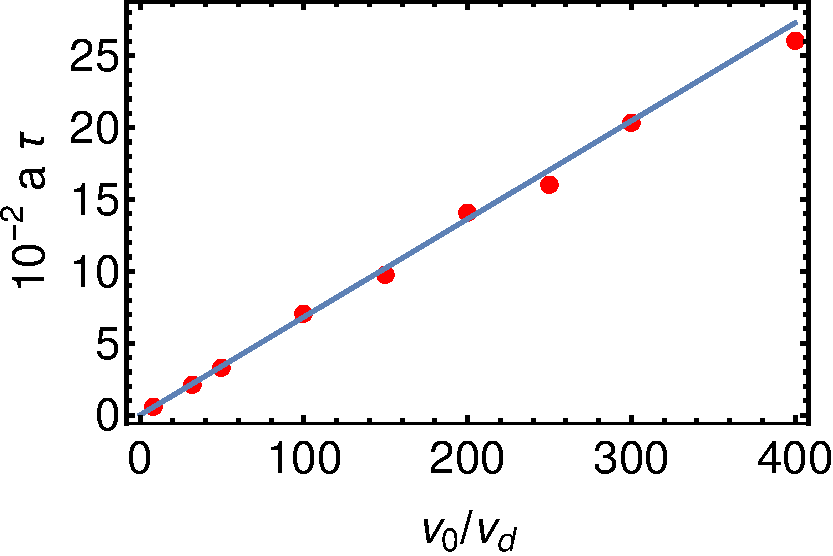
\includegraphics[width=0.48\linewidth]{Figures/asym_fig_t_a_param1.pdf}
  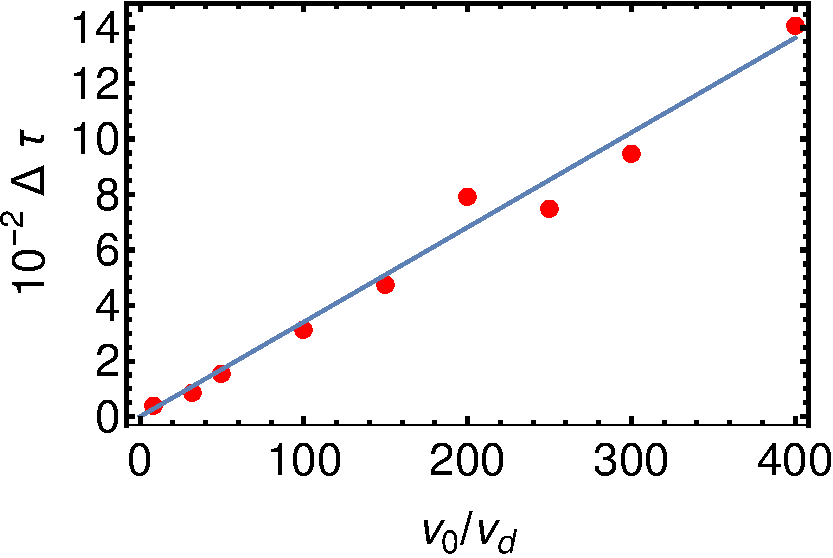
\includegraphics[width=0.48\linewidth]{Figures/asym_fig_t_a_param2.pdf}
  \end{center}
  \caption{Asymmetric ${\cal T/A}$ device with symmetry VIII: comparison between numerically achieved parameters (red dots) and approximated parameters (blue, solid lines) versus velocity $v_0$.
  (a) Height of Rabi frequency $a$, (b) detuning $\Delta$.
  \label{fig_t_a_param}}
\end{figure}
% ------------------------------------------------------------------------------

%
%
%
%

%
%
\section{Discussion\label{sec:chapter3_Discussion}}

% Non-Hermitian Hamiltonians display many interesting phenomena which are
% impossible for a  Hermitian Hamiltonian  acting on the same Hilbert space. In particular, in the Hilbert space of
% a single, structureless particle on a line formed by square integrable normalizable functions, Hermitian Hamiltonians do not allow, within a linear theory, for asymmetric scattering transmission and reflection coefficients.
% % for right/left incidence of a particle off a potential center.
% However,
% non-Hermitian Hamiltonians do.

Since devices of technological interest, such as one-way filters for transmission or reflection, one-way barriers, one-way mirrors, and others, may be built based on the asymmetric scattering response of non-Hermitian Hamiltonians, there is both fundamental
interest and applications in sight to implement Non-Hermitian scattering Hamiltonians. The results in this chapter are a step forward in that direction, specifically I propose a quantum-optical implementation of potentials with asymmetric scattering response.
They are non-local and non-PT symmetrical, which allows for asymmetric transmission.

In general the chosen Hilbert space may  be regarded as a subspace of a larger space. For example,  the space of a ``structureless particle'' in 1D is the ground-state subspace
for a particle with internal structure, consisting of two-levels in the simplest scenario.
It is then possible to regard the Non-Hermitian physics in the reduced space
as a projection of the larger space, which may itself be driven by a  Hermitian or a Non-Hermitian Hamiltonian.
I have seen the Hermitian option in our examples, where I assumed a zero decay constant, $\gamma=0$, for the excited state.
A non-zero $\gamma$ implies  a Non-Hermitian  Hamiltonian in the larger two-level space. The description may still be
enlarged,  including  quantized field modes to account for the atom-field interaction with a Hermitian Hamiltonian.
As an outlook, depending on the application, there might be the need for a more fundamental and detailed descriptive level. Presently I discuss the desired physics (i.e., the scattering asymmetries) at the level of the smallest 1D space of the ground state, while taking refuge in the
two-level space to find a feasible physical implementation.
